% !TeX root = document.tex
\chapter{Maschinelle Werteanpassung}

Es ist schwer menschliche Werte in Computersystemen zu programmieren (siehe Kapitel \ref{Werte}), deshalb haben \citeauthor{irving_ai_2018} einen anderen Ansatz der Werteanpassung verfolgt: die des menschlichen Feedbacks (eng. \emph{human-feedback-loop}, siehe Abbildung \ref{humanfeedbackimg}).

Hierbei fragt eine KI einen menschlichen Operator nach der Nützlichkeit und Sicherheit ihres Verhaltens. Bei schlechter Bewertung passt die KI ihre Lösungsfunktion an, somit ist keine riskante Zielsetzung im Vorhinein notwendig. \vgl{christiano_deep_2017} Dies funktioniert so lange gut, bis der Operator nicht mehr in der Lage ist, das Handeln der KI nachzuvollziehen und zu beurteilen. \vgl[1-2]{irving_ai_2018}

\begin{figure}
  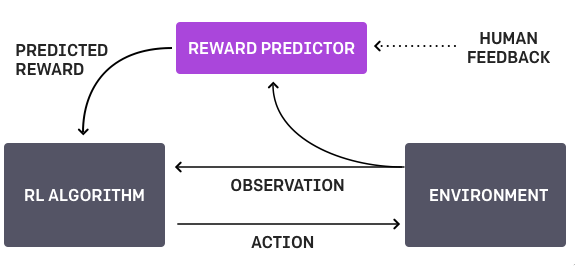
\includegraphics{humanfeedback}
  \caption{Repräsentation einer human-feedback-loop}
  \label{humanfeedbackimg}
\end{figure}


%Was ist eine Reward function?
%Eine Nutzfunktion ist 


%Ein Algorithmus einer sicheren AKI muss die folgenden Probleme lösen:
%\begin{enumerate}
%\item Negative Effekte durch eine fehlerhaft definierte Nutzfunktion zur Feststellung der Ziele
%\item Eine AKI könnte eine Problemstellung mit der Intention, sie wieder lösen zu können, verschlimmern. (Ein Staubsaugroboter, der Staub herstellt, um ihn dann wieder aufsaugen zu können.) \vgl[1-2]{hadfield-menell_inverse_2017}
%\end{enumerate}

%https://80000hours.org/articles/ai-safety-syllabus/
%\vgl{yudkowsky_intelligence_2013}
%\section{Wertekodierung in einer Programmiersprache}
%KOMMENTAR: Complexity of Value Theory
%\subsection{Statische Wertekodierung}
%\subsection{Dynamisch-maschinelle Werteanpassung}
%
%\section{Mensch-Maschinen-Interface}
%\section{Hirnemulation}
%\section{Friendly AI}



%%% Local Variables:
%%% mode: latex
%%% TeX-master: "document"
%%% End:
